\subsection{Wymagania funkcjonalne i niefunkcjonalne}
\begin{enumerate}
    \item Wymagania funkcjonalne
    \begin{enumerate}
        \item Użytkownik zakłada konto
        \item Użytkownik loguję się
        \item Użytkownik przegląda zasoby
        \item Użytkownik sprawdza dostępność danego zasobu
        \item Użytkownik sprawdza informację o zasobie
        \item Pracownik dodaje zasoby
        \item Pracownik usuwa zasoby
        \item Pracownik zarządza zasobami
        \item Pracownik zmienia ilość dostępnych zasobów
        \item Pracownik sprawdza status danego egzemplarza
        \item Pracownik zatwierdza lub odrzuca prośbę o wypożyczenie egzemplarza
        \item Pracownik zatwierdza lub odrzuca prośbę o przedłużenie terminu wypożyczenia egzemplarza
        \item Pracownik zarządza egzemplarzami zasobów
        \item Pracownik odnotowuje zwrot wypożyczonego egzemplarza
        \item Klient przegląda wypożyczone przez niego zasoby
        \item Klient zgłasza prośbę o wypożyczenie egzemplarza zasobu
        \item Klient zgłasza prośbę o przedłużenie terminu wypożyczenia
    \end{enumerate}
    \item Wymagania niefunkcjonalne
    \begin{enumerate}
        \item Aktualizacja zasobów jest rejestrowana w bazie danych
        \item System jest przyjazny i prosty w obsłudze
        \item System zapewnia bezpieczeństwo danych użytkownika
        \item System chroni dane klientów
        \item System informuje klienta o odmowie wypożyczenia egzemplarza
        \item Klienci zgłaszają dowolną ilość próśb o wypożyczenie
        \item Użytkownicy mają różne uprawnienia
        \item System jest uruchamiany na popularnych systemach
    \end{enumerate}
\end{enumerate}

\subsection{Diagram przypadków użycia}
\begin{figure}[H]
    \centering
    \resizebox{\columnwidth}{!}{%
    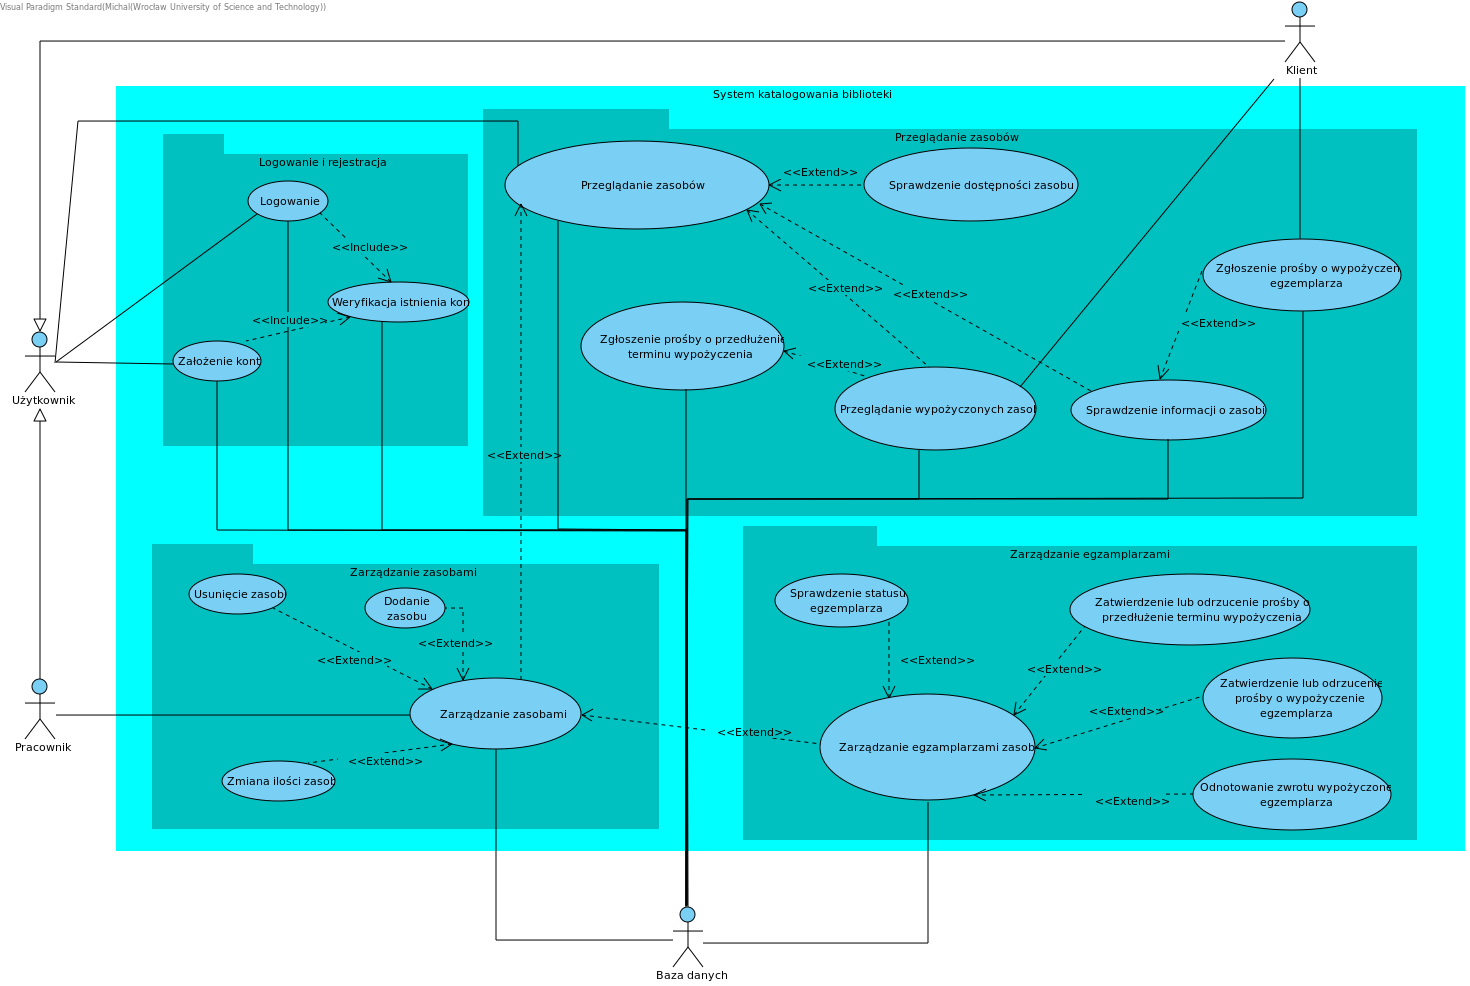
\includegraphics{Img/Use Case Diagram old.png}%
    }
    \caption{Diagram przypadków użycia}
\end{figure}


\subsection{Opis scenariuszy}
\begin{figure}[H]
    \centering
    \resizebox{\columnwidth}{!}{%
    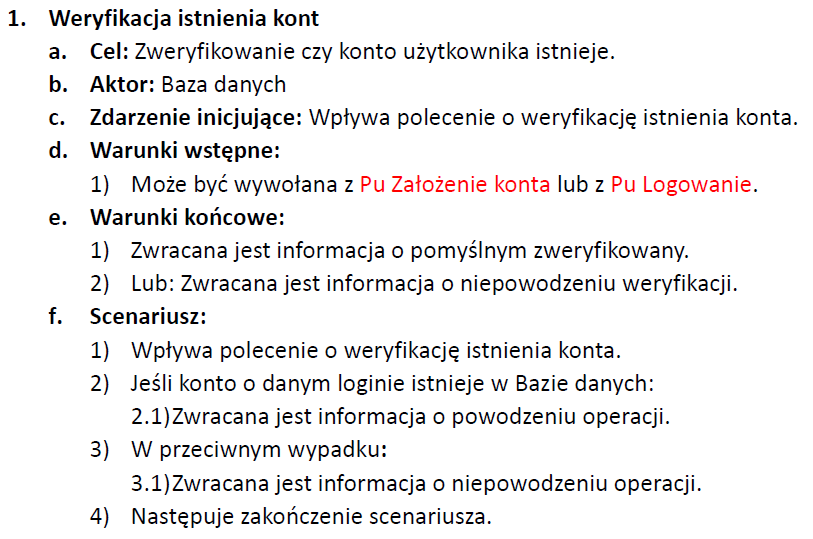
\includegraphics{Img/Scenariusze/1.png}%
    }
\end{figure}

\begin{figure}[H]
    \centering
    \resizebox{\columnwidth}{!}{%
    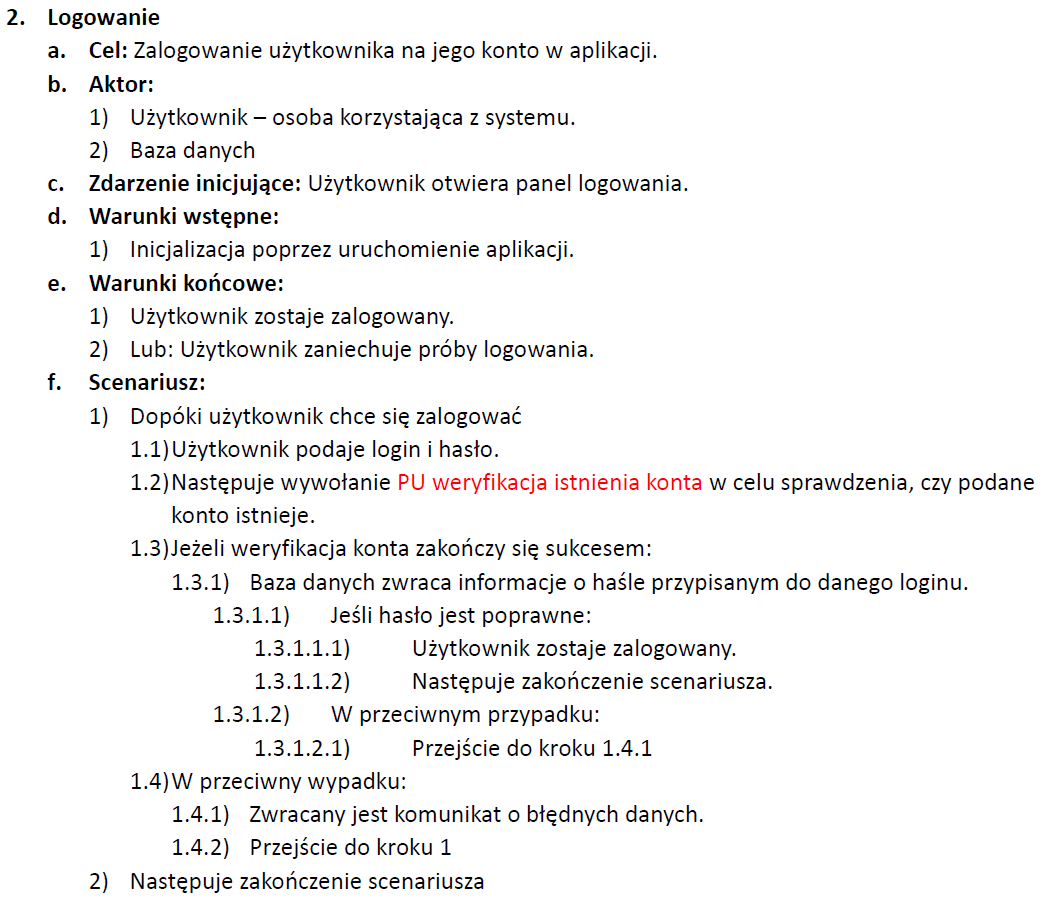
\includegraphics{Img/Scenariusze/2.png}%
    }
\end{figure}

\begin{figure}[H]
    \centering
    \resizebox{\columnwidth}{!}{%
    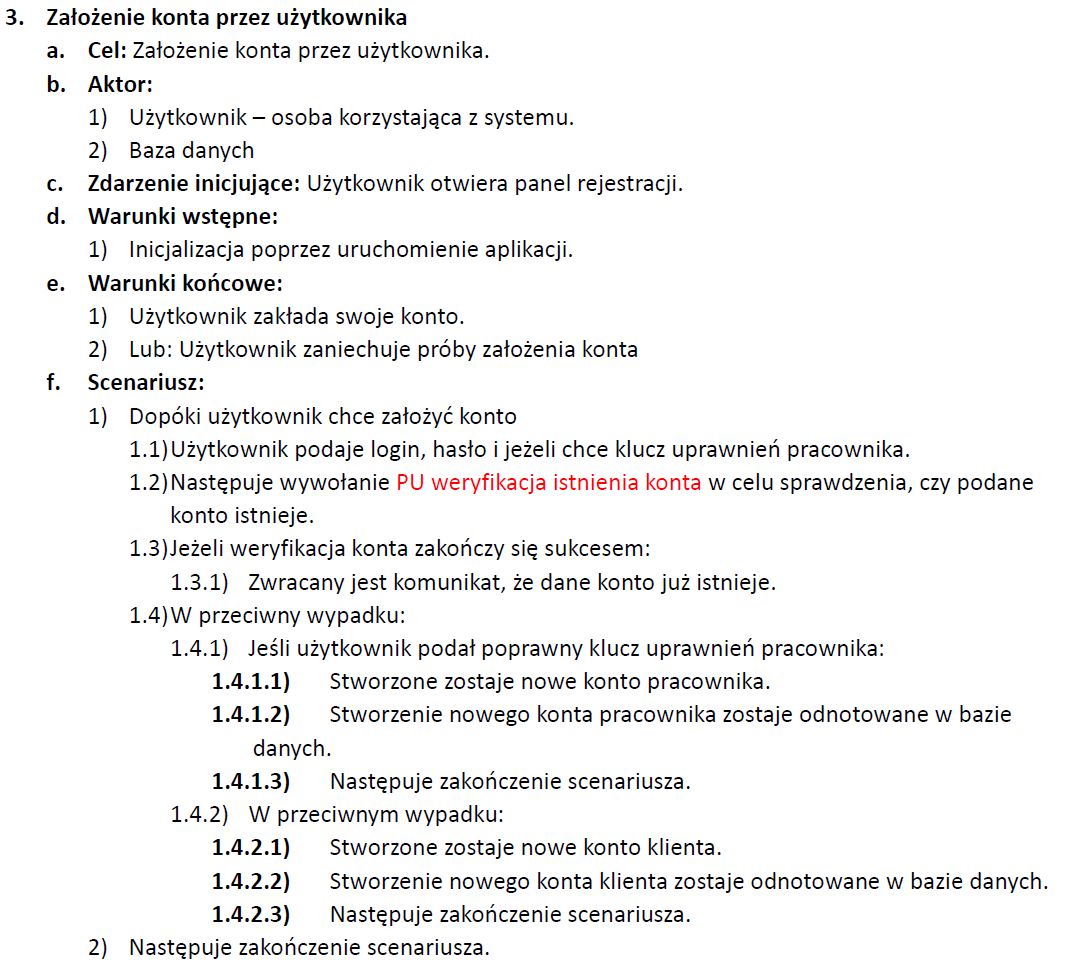
\includegraphics{Img/Scenariusze/3.png}%
    }
\end{figure}

\begin{figure}[H]
    \centering
    \resizebox{\columnwidth}{!}{%
    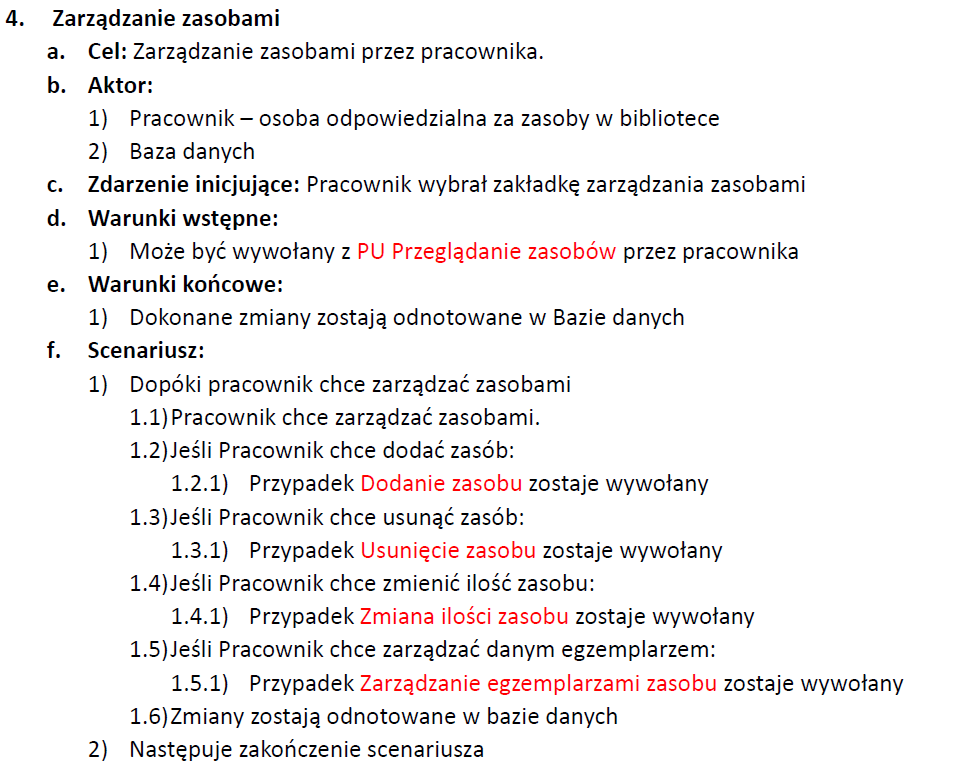
\includegraphics{Img/Scenariusze/4.png}%
    }
\end{figure}

\begin{figure}[H]
    \centering
    \resizebox{\columnwidth}{!}{%
    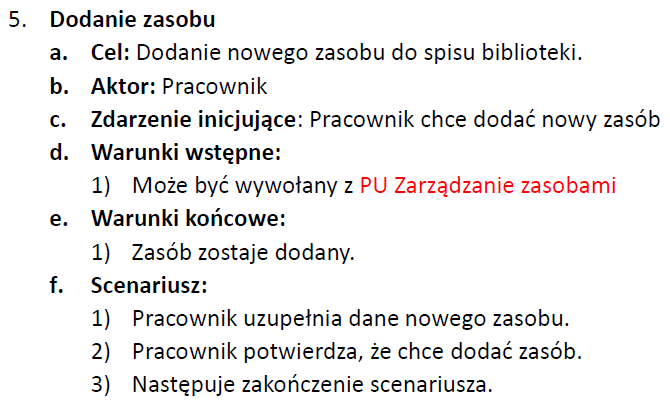
\includegraphics{Img/Scenariusze/5.png}%
    }
\end{figure}

\begin{figure}[H]
    \centering
    \resizebox{\columnwidth}{!}{%
    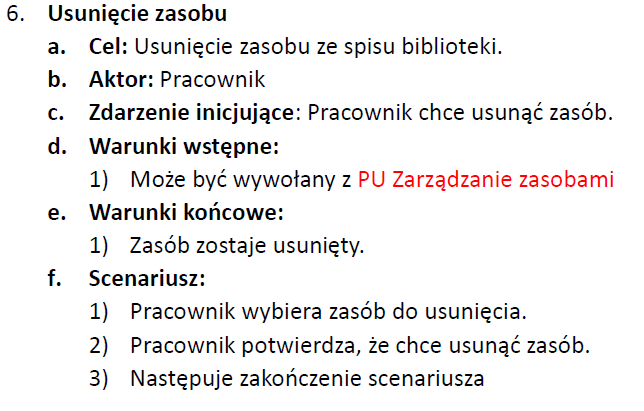
\includegraphics{Img/Scenariusze/6.png}%
    }
\end{figure}

\begin{figure}[H]
    \centering
    \resizebox{\columnwidth}{!}{%
    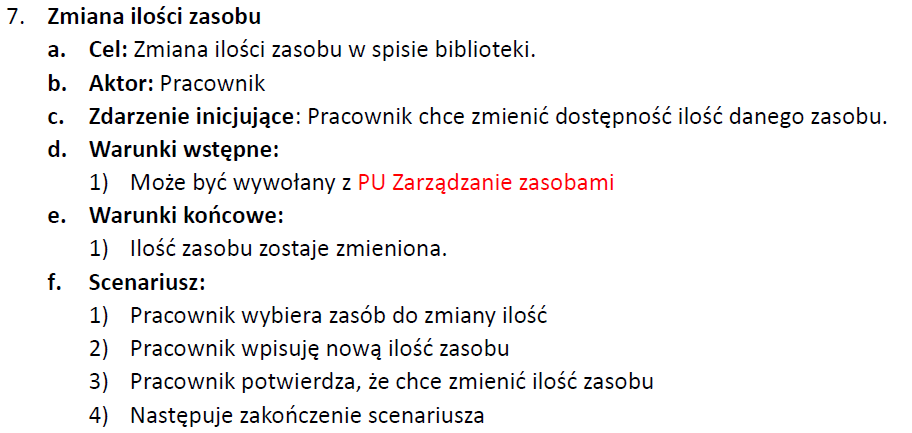
\includegraphics{Img/Scenariusze/7.png}%
    }
\end{figure}

\begin{figure}[H]
    \centering
    \resizebox{\columnwidth}{!}{%
    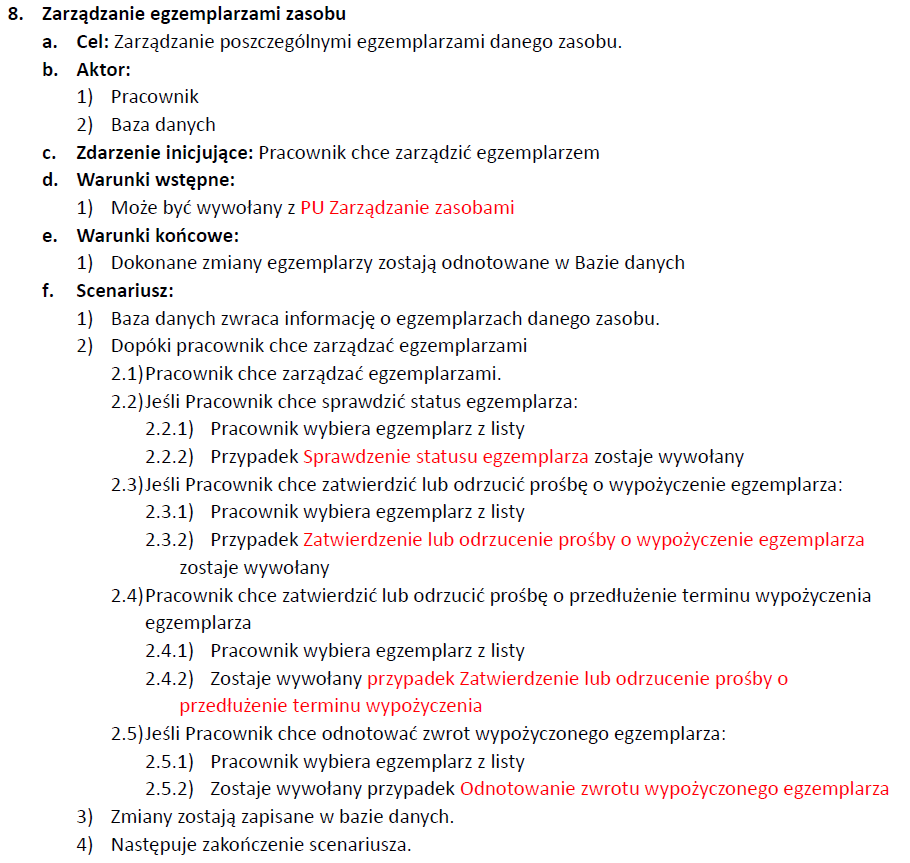
\includegraphics{Img/Scenariusze/8.png}%
    }
\end{figure}

\begin{figure}[H]
    \centering
    \resizebox{\columnwidth}{!}{%
    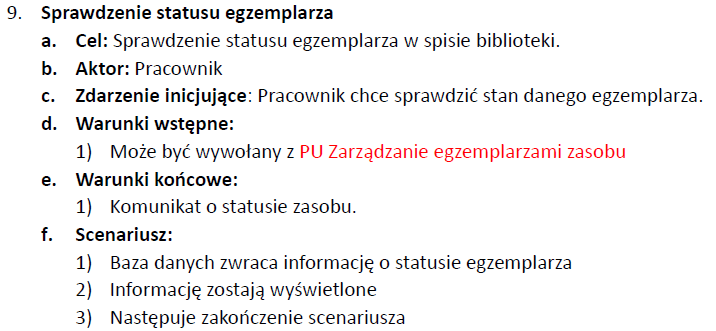
\includegraphics{Img/Scenariusze/9.png}%
    }
\end{figure}

\begin{figure}[H]
    \centering
    \resizebox{\columnwidth}{!}{%
    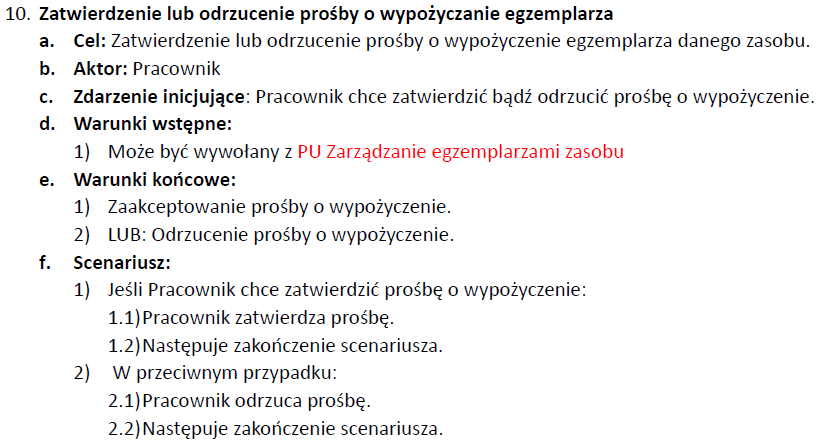
\includegraphics{Img/Scenariusze/10.png}%
    }
\end{figure}

\begin{figure}[H]
    \centering
    \resizebox{\columnwidth}{!}{%
    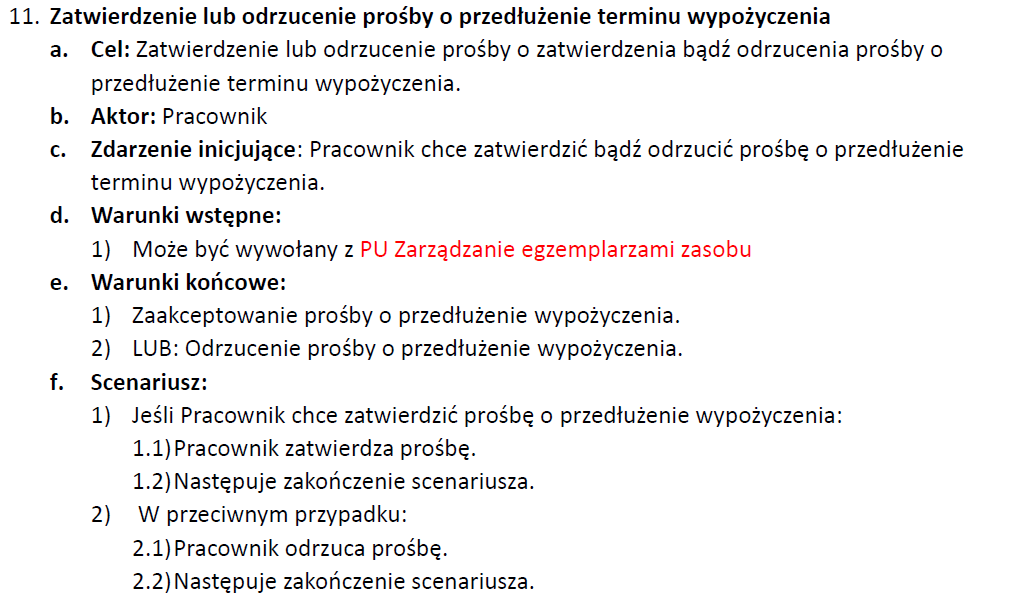
\includegraphics{Img/Scenariusze/11.png}%
    }
\end{figure}

\begin{figure}[H]
    \centering
    \resizebox{\columnwidth}{!}{%
    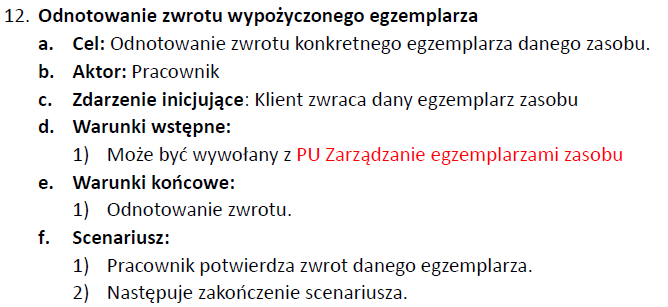
\includegraphics{Img/Scenariusze/12.png}%
    }
\end{figure}

\begin{figure}[H]
    \centering
    \resizebox{\columnwidth}{!}{%
    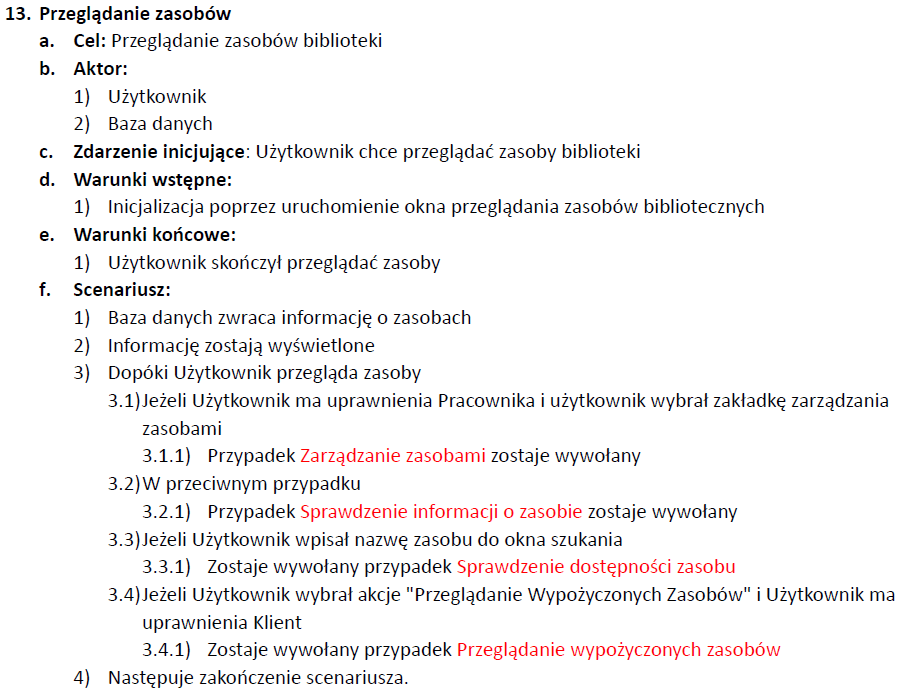
\includegraphics{Img/Scenariusze/13.png}%
    }
\end{figure}

\begin{figure}[H]
    \centering
    \resizebox{\columnwidth}{!}{%
    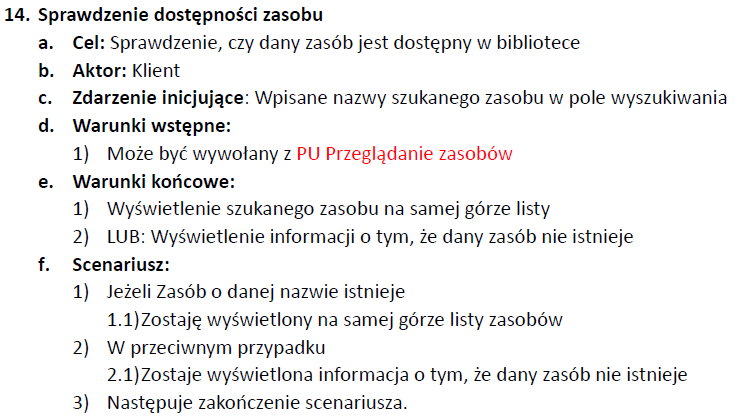
\includegraphics{Img/Scenariusze/14.png}%
    }
\end{figure}

\begin{figure}[H]
    \centering
    \resizebox{\columnwidth}{!}{%
    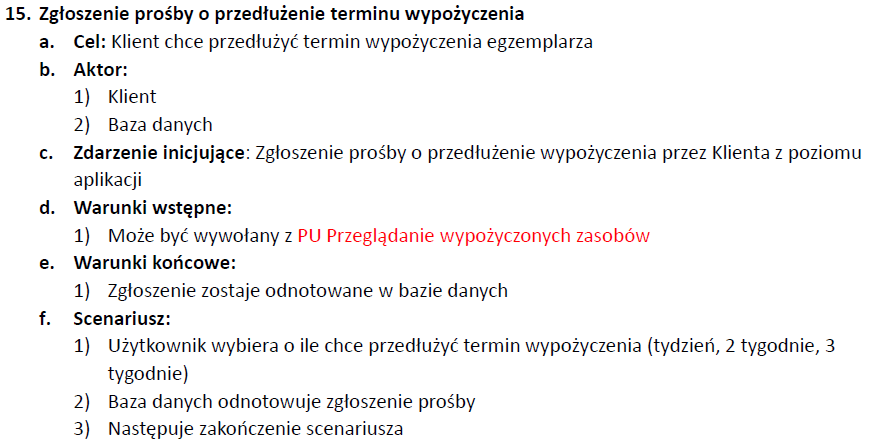
\includegraphics{Img/Scenariusze/15.png}%
    }
\end{figure}

\begin{figure}[H]
    \centering
    \resizebox{\columnwidth}{!}{%
    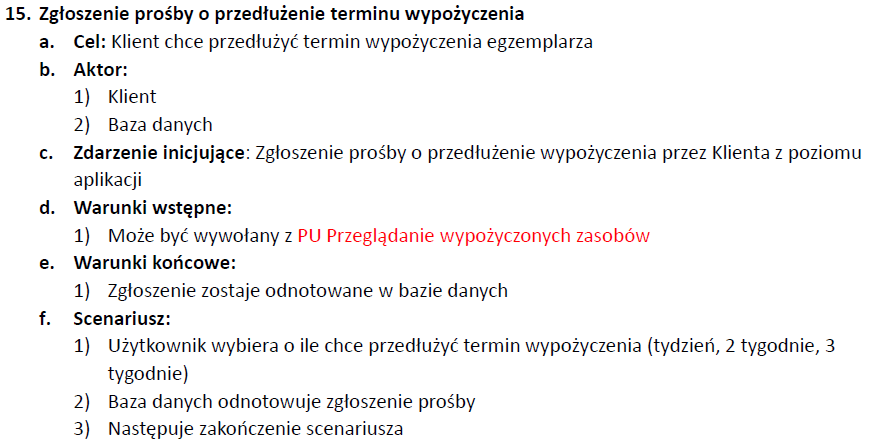
\includegraphics{Img/Scenariusze/15.png}%
    }
\end{figure}

\begin{figure}[H]
    \centering
    \resizebox{\columnwidth}{!}{%
    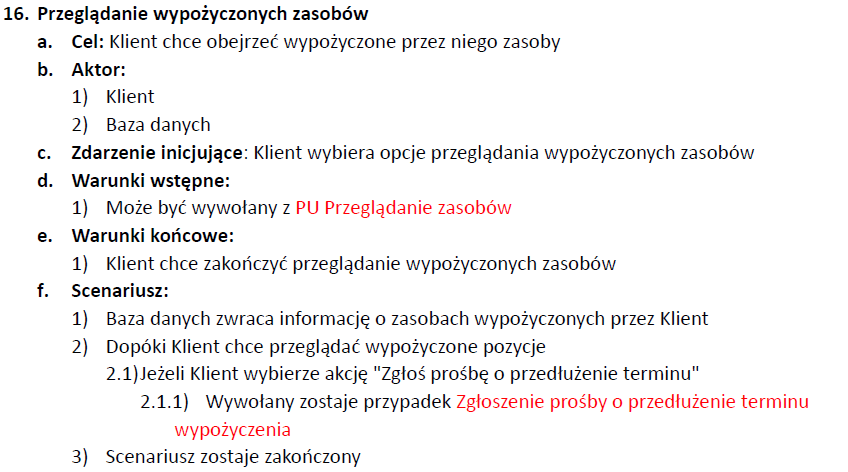
\includegraphics{Img/Scenariusze/16.png}%
    }
\end{figure}

\begin{figure}[H]
    \centering
    \resizebox{\columnwidth}{!}{%
    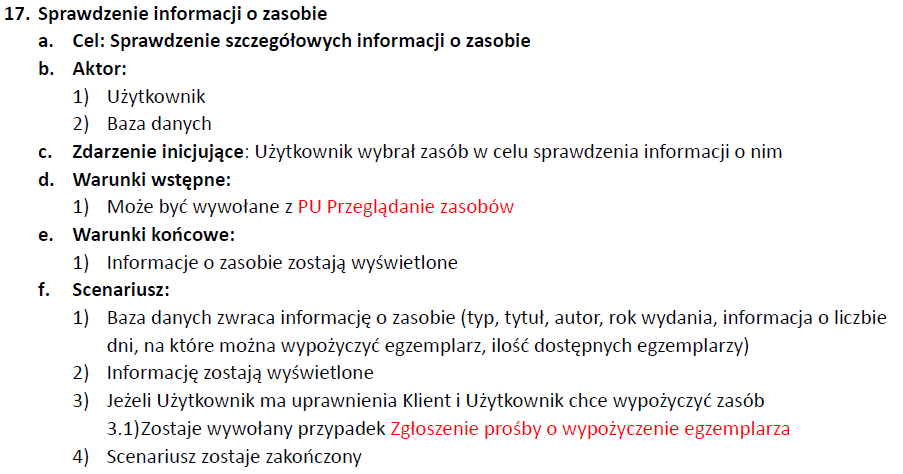
\includegraphics{Img/Scenariusze/17.png}%
    }
\end{figure}

\begin{figure}[H]
    \centering
    \resizebox{\columnwidth}{!}{%
    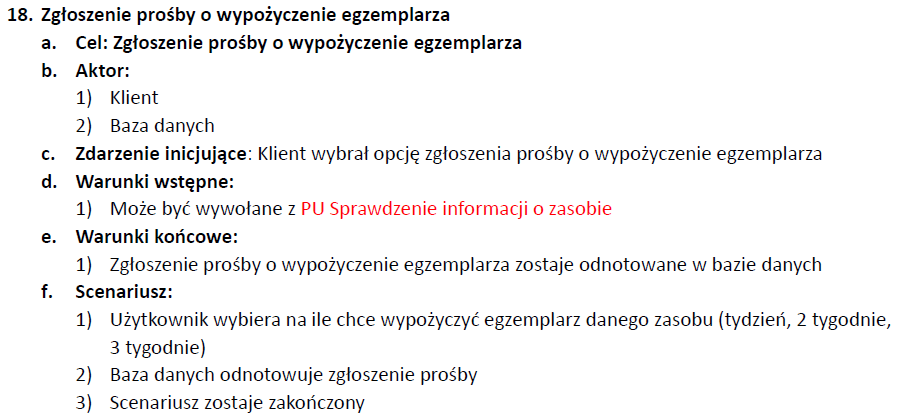
\includegraphics{Img/Scenariusze/18.png}%
    }
\end{figure}


\subsection{Diagram ERD}
\begin{figure}[H]
    \centering
    \resizebox{\columnwidth}{!}{%
    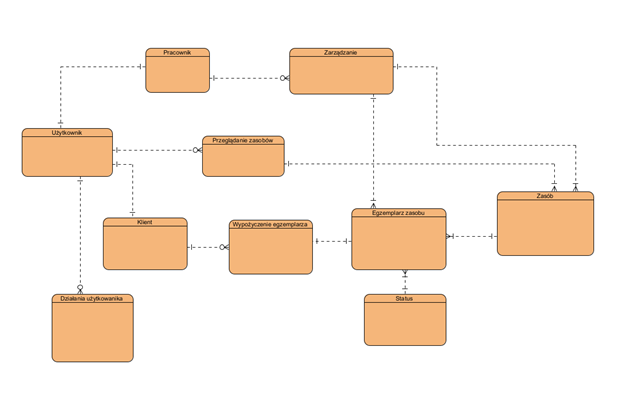
\includegraphics{Img/erd1.png}%
    }
    \caption{Diagram ERD}
\end{figure}